\documentclass[10pt, english]{report}

\usepackage{hyperref}

\usepackage{float}

\usepackage{subcaption}
\usepackage[export]{adjustbox}
\usepackage{wrapfig}
%encoding
%--------------------------------------
\usepackage[utf8]{inputenc}
\usepackage[T1]{fontenc}
%--------------------------------------

%French-specific commands
%--------------------------------------
\usepackage{babel}
\usepackage[autolanguage]{numprint}
%--------------------------------------

%Hyphenation rules
%--------------------------------------
\usepackage{hyphenat}
\hyphenation{mathéma-tiques récu-pérer}
%--------------------------------------

%Maths box
%--------------------------------------
\usepackage{amsmath}
\usepackage[most]{tcolorbox}

\tcbset{colback=yellow!10!white, colframe=red!50!black, 
	highlight math style= {enhanced, %<-- needed for the ’remember’ options
		colframe=red,colback=red!10!white,boxsep=0pt}
}
%--------------------------------------

%code blocs
%--------------------------------------

\usepackage{listings}
\usepackage{xcolor}

\definecolor{codegreen}{rgb}{0,0.6,0}
\definecolor{codegray}{rgb}{0.5,0.5,0.5}
\definecolor{codepurple}{rgb}{0.58,0,0.82}
\definecolor{backcolour}{rgb}{0.95,0.95,0.92}

\lstdefinestyle{mystyle}{
	backgroundcolor=\color{backcolour},   
	commentstyle=\color{codegreen},
	keywordstyle=\color{magenta},
	numberstyle=\tiny\color{codegray},
	stringstyle=\color{codepurple},
	basicstyle=\ttfamily\footnotesize,
	breakatwhitespace=false,         
	breaklines=true,                 
	captionpos=b,                    
	keepspaces=true,                 
	numbers=left,                    
	numbersep=5pt,                  
	showspaces=false,                
	showstringspaces=false,
	showtabs=false,                  
	tabsize=2
}

\lstset{style=mystyle}
%--------------------------------------

\usepackage[margin=2cm]{geometry}
\usepackage{graphicx}

\title{
	
\includegraphics[scale=1]{img/logo.png}\\[4cm]
	\huge\textbf{Natural Language Processing for Fact-Checking and Claim Assessment}\\[1cm]
	\Large{Intermediate report of project advancement} \\[4cm]
}
\author{
	Othman EL HOUFI\\
	Dimitris KOTZINOS \\[0.5cm]
	\textbf{MSc Research in Data Science \& Machine Learning} \\[1.5cm]
}

\date{\today}

\begin{document}
	
	%%%%%TITLE%%%%%
	\begin{titlepage}
		\maketitle
	\end{titlepage}

\chapter*{Abstract}
As false information and fake news are propagating though out the internet and social networks, the need of fact-checking operations becomes necessary in order to maintain a truthful digital environment where general information can be reliably exploited whether in politics, finance and other domains. The need of this online claim assessment comes from the fact that fake news and false information can have a big negative impact on politics, economy (2016 USA Elections) and public health (COVID-19).\\ 
A number of solutions have been proposed to deal with this problem and limit the spread of false information, both manual and automatic. Of course the manual approaches done on websites such as \textit{PolitiFact.com}, \textit{FactCheck.org} and \textit{Snopes.com} don't construct a viable solution for the long term as the speed and scale of information propagation increase exponentially rendering this manual fact-checking operation where human fact-checkers can't scale up at the same rate limited and incapable of solving the problem.\\
Here, we present our contribution in this regard: an automated solution for fact-checking using Wikipedia's articles for claim verification. The algorithm uses NLP techniques \cite{lazarski2021using} in order to extract the so-called claim from the user input, then, using Wikipedia's API, it retrieves all the relevant articles and assesses with a degree of confidence if the claim is true, false or unable to decide due to lack of information showing evidence (sentences in articles) and probabilities for each resulted case.\\[1cm]

\textbf{Keywords:} Natural Language Processing, Wikipedia, Information retrieval, Text processing, Natural Language Inferencing, Fact-Checking, Document retrieval, Sentence retrieval, Fake-news.

%%%%%TABLE OF CONTENT%%%%%
\tableofcontents

\chapter{Introduction}
\section{Project Context}

From a social and psychological perspective, humans have been proven irrational and vulnerable when differentiating between truth and false news (typical accuracy ranges between 55\% and 58\%) \cite{zhou2019fake}, thus fake news obtain public trust relatively easier than truthful news because individuals tend to trust fake news after repeated exposure (\textit{Validity effect}), or if it confirms their pre-existing beliefs (\textit{Confirmation bias}), or simply due to the obligation of participating socially and proving a social identity (\textit{Peer pressure}). The social sciences are still trying to comprehend the biological motivations that makes fake news more appealing to humans.\\

On the other hand, the growth of social media platforms resulted in a huge acceleration of news spreading whether true or false. As of Aug. 2017, 67\% \cite{zhou2019fake} of Americans get their news from social media. These platforms even give the user the right to share, forward, vote and participate to online discussions. All of this made the problem of fake news spreading more and more dangerous, our economies for example, are not robust to the spread of falsity, false rumors have affected stock prices and the motivations for large-scale investments, as we witnessed after a false tweet claimed that Barack Obama was injured in an explosion which caused \$130 billion drop in stock value \cite{vosoughi2018spread}. Another recent example is related to public health where rumors about COVID-19 vaccines and drug companies influenced people in their decision on getting vaccinated.\\

That being said, is there a way to monitor the spread of fake news through social media? Or more specifically, how can we differentiate between fake news and truthful news, and at what level of confidence can we do that?\\

From a computer engineering perspective, different approaches were studied:

\begin{itemize}
\item \textbf{Knowledge-based Fake News Detection \cite{chernyavskiy2021whatthewikifact}:} a method aims to assess news authenticity by comparing the knowledge extracted from to-be verified news content with known facts, also called fact-checking.
\item \textbf{Style-based Fake News Detection \cite{przybyla2020capturing}:} focuses on the style of writing, i.e. the form of text rather than its meaning.
\item \textbf{Propagation-based Fake News Detection \cite{shu2020hierarchical}:} a principled way to characterize and understand hierarchical propagation network features. We perform a statistical comparative analysis over these features, including micro-level and macro-level, of fake news and true news.
\item \textbf{Credibility-based Fake News Detection \cite{sitaula2020credibility}:} the information about authors of news articles can indicate news credibility and help detect fake news.
\end{itemize}

In this project we will focus on the method of \textbf{Knowledge-based Fake News Detection} also called \textbf{Fact-Checking}. The goal is not to implement an algorithm that scans social networks for real time fake news detection, but rather we will create a model that can assess with a degree of confidence the truthfulness or falseness of a claim given by a user as an input by exploiting Wikipedia's articles \cite{trokhymovychnatural} as a source of true knowledge and export evidence that validates or refutes the subjected claim.

\section{Use case scenario}
Suppose that while browsing the internet or talking to people you come across a claim that says \textit{"The former U.S president John F. Kennedy died in September 22, 1963"}, as it is a general truth and not a relative truth it should be easier to verify the validity of this claim as well as find evidence that proves it.\\
Using the platform we will create, you can simply write the claim you like to verify with no regards to a specific linguistic rule, the model will extract relevant articles from Wikipedia using an API, then it retrieves sentences relative to your claim and apply a comparison in order to assess if the claim is True, False, or Not Enough Information as well as giving a percentage of confidence and evidence of the results that were processed straight from Wikipedia's database.\\
Combing back to our example, the model should return that \textit{"John F. Kennedy died in November 22, 1963"} so the input claim is false.

\begin{figure}[H]
	\centering
	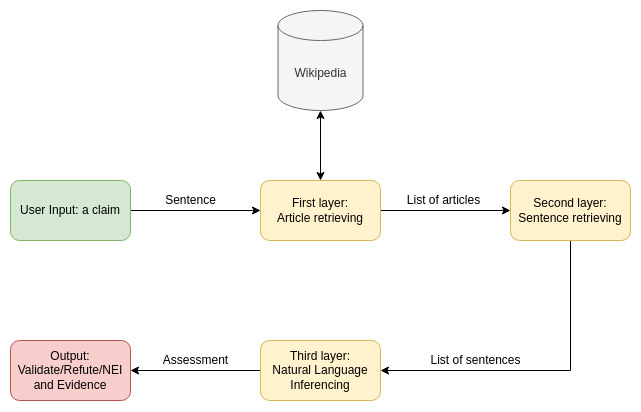
\includegraphics[scale=0.6]{img/use_case.png}
	\caption{General Model Processing Pipeline}
\end{figure}


\chapter{Identified challenges and solutions}
\section{Fact-Checking challenges}
In order for the model to work each layer/part of the system must answer to a specific task, the combination of results made by each layer constructs a robust model that is able with a degree of confidence to fact-check a claim as well as present evidence of the assessment. Although for each layer to work as intended we must find solutions to these challenges:\\

\begin{itemize}
	\item \textbf{Claims Spotting:} the model must be robust to linguistic changes, we must deal with different phrasing for the same or similar claims. For every "reasonable" input we must extract the target claim.
	\item \textbf{Articles Retrieving:} as Wikipedia holds millions of articles, the model must look for a limited number of relative articles to the input claim with an order of degree of correlation.
	\item \textbf{Time Recording:} relative articles in Wikipedia can be outdated, for example Britain belongs to the European Union is an outdated knowledge. The model must be sensitive to the timestamps of articles.
	\item \textbf{Sentences Retrieving:}  in each article retrieved from Wikipedia's database we must extract sentences relative to our input claim in order to apply a "kind of" comparison as well as present the winning sentences as evidence to the user.
	\item \textbf{Sentence Comparison:} here we must create a model or use a pre-existing natural language inferencing model in order to compare retrieved sentences from Wikipedia's articles and the input claim. 
	\item \textbf{Credibility Evaluation:} not all informations in Wikipedia are true.
\end{itemize}

These can be regarded as main challenges of our Fact-Checking project, but, evidently, other problems can be presented for example the verifiability of claims, not all claims can be verifiable, especially if it is an personal opinion or a personal belief, in this case the model must not give a True or False assessment but it should tell the user that there is not enough information (NEI) to make such an assessment.

\section{Potential Datasets}


\section{Related work and solutions}
\subsection{Language model based fake news detection \cite{lee2020language}}

\subsection{Styled based fake news detection \cite{przybyla2020capturing}}
A study done by \textit{Piotr Przybyła} named \textit{Capturing the Style of Fake News} in 2020 from Institute of Computer Science, Polish Academy of Sciences, in order to detect fake news or in other words assess the credibility of an article by looking at the style of writing rather than the meaning of the words and sentences.\\
The purpose of this study was to prove that general-purpose text classifiers, despite their good performance when evaluating simplistically, they overfit to sources of documents in training data. In contrast to this method, a truly style-based prediction that uses an analysis of the stylometric model shows that it focuses on sensational and affective vocabulary, known to be typical for fake news.\\

Fake news sources usually attempt to attract attention for short-time financial or political goal \cite{allcott2017social} rather than to build a long-term relationship with the reader, in this perspective, the language used by these sources tend to be informal, sensational and affective \cite{bakir2017fake}. This can be used to build a classifier for indicating low credibility.\\

First of all they started by gathering a corpus of 103,219 documents from 223 online sources labeled by media experts like \textit{PolitiFact} and \textit{Pew Research Center}. Then they designed two models: a neural network and a model based on features used in stylometric analysis. This has a purpose to demonstrate that the stylometric features based model captures the affective language elements.\\

\begin{figure}[H]
	\centering
	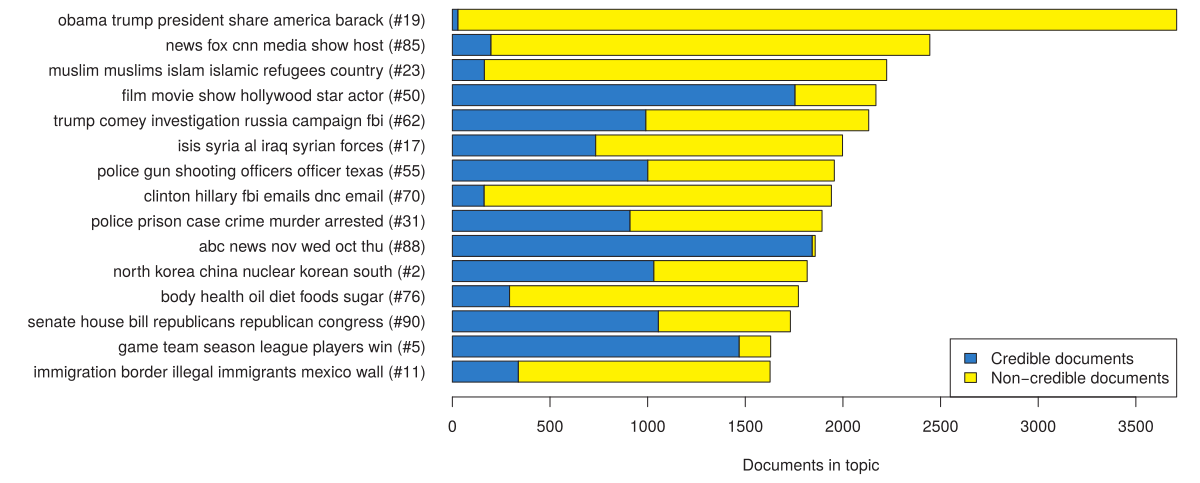
\includegraphics[scale=0.4]{img/documents_in_topic.png}
	\caption{From Piotr Przybyła paper - The largest 15 LDA (Latent Dirichlet Allocation) topics in the corpus, each shown with the six most significant keywords, an identifier and bars illustrating number of credible and non-credible documents associated with it}
\end{figure}

\textbf{Stylometric classifier:} the architecture of this classifier is generally based on a collection of stylystic features followed by a linear modeling. The features are: 
	\begin{itemize}
	\item number of sentences, average sentence length (in words) and average word length (in characters),
	\item number of words matching different letter case schemes (all lower case, all upper case, just first letter upper case, other), represented as counts normalized by the document length,
	\item frequencies of POS uni-grams, bi-grams and trigrams, represented as counts normalized by the document length (if present in at least 5 documents),
	\item frequencies of words belonging to the 182 word categories in the expanded GI dictionary, represented as counts normalized by the document length.
	\end{itemize}

\textbf{Neural network classifier:} the applied solution was BiLSTMAvg a neural network with architecture based on elements used in natural language processing, i.e. word embeddings \cite{mikolov2013efficient} and bidirectional LSTM (Hochreiter and Schmidhuber 1997). The following layers are included:
	\begin{itemize}
	\item An embedding layer, representing each token using a 300-dimensional word2vec vector trained on Google News,
	\item Two LSTM layers, forward and backward, representing each sentence by two 100-dimensional vectors (output of the last cell in a sequence),
	\item A densely-connected layer, reducing the dimensionality to 2 and applying softmax to compute class probability,
	\item An averaging layer, representing each document’s class probability scores by averaging the scores for all its sentences.
	\end{itemize}
The neural network is implemented and trained in TensorFlow for 10 epochs with sentence length limited to 120 tokens and document length limited to 50 sentences.\\

In order to understand if general-purpose text classifiers can capture document style without overfitting to features like the source or topic of document and to compare with the two classifiers they created, they evaluated two baseline models: bag of words and BERT.\\

The evaluation protocol consisted on running the model learning and prediction in a 5-fold cross validation (CV) scenario and comparing it's output to target labels. They used accuracy as a metric of evaluation rather than precision or recall.

\begin{figure}[H]
	\centering
	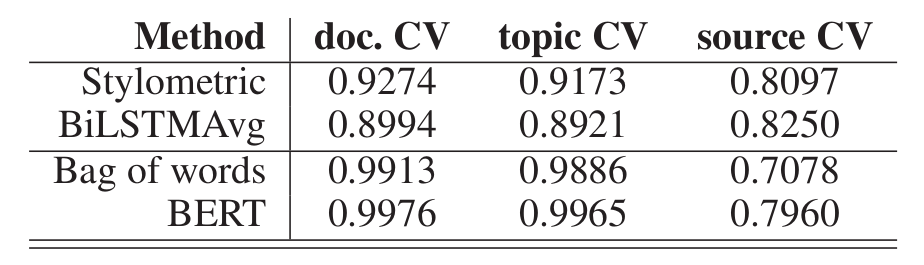
\includegraphics[scale=0.3]{img/styled_model_result.png}
	\caption{From Piotr Przybyła paper - Classification accuracy of our stylometric and neural classifiers compared to baselines in three evaluation scenarios, simulating, respectively, a new document from known sources and topics, a document from unknown topic and a document from unseen source}
\end{figure}

The obtained results shows that stylometric based classifier loses 10\% of the accuracy on unseen sources even if it has more consistent performance over evaluation scenarios. Piotr Przybyła explains this drop in accuracy by assuming that the model specialize in the style of individual sources rather than the general style of fake news. Nevertheless, he was able to prove that his model takes into account the affective words in order to classify fake news.
\subsection{Knowledge graph based fake news detection \cite{mayank2021deap}}
Studying the \textit{"DEAP-FAKED"} paper published in 2021 by \textit{Mohit Mayank}, \textit{Shakshi Sharma} and \textit{Rajesh Sharma}, it turned out that by exploiting techniques related to network analysis, Natural Language Processing (NLP) and the implementation of Graph Neural Networks (GNNs) we can detect fake news with an F1 score of 88\%.\\

The \textit{"DEAP-FAKED"} consists of three individual components:

\begin{itemize}
\item \textbf{News encoder:} this component performs the contextual encoding of news title. trying both unidirectional and bidirectional sequence encoders, they implemented a 2-layer stacked biLSTM as the main subcomponent the news encoder.
\item \textbf{Entity encoder:} this component identifies the named entities present in the news title and encodes the individual entities using knowledge graph (KG).
For example, a news title with text \textit{"US Officials See No Link Between Trump and Russia"}, contains two entities \textit{"Trump"} of person type and \textit{"Russia"} of geolocation type.
The framework includes relevant entities in the news then encodes them. They used Wikidata, an open-source KG, as the source to match the entities and ComplEx KG embedding technique to embed entities.
\item \textbf{Classification Layer:} this component consolidates the news encoder's and entity encoder's representations to perform the final downstream Fake News classification learning.
In this framework, the two representations are concatenated to create a super representation of the news content and entities. This representation is then passed to further non-linear activated layers with decreasing layer dimensionality. The final layer consolidated the information into a single dimension which is activated by a sigmoid layer, where the final output represents the probability of the news as either true or fake.
\end{itemize}

\begin{figure}[H]
	\centering
	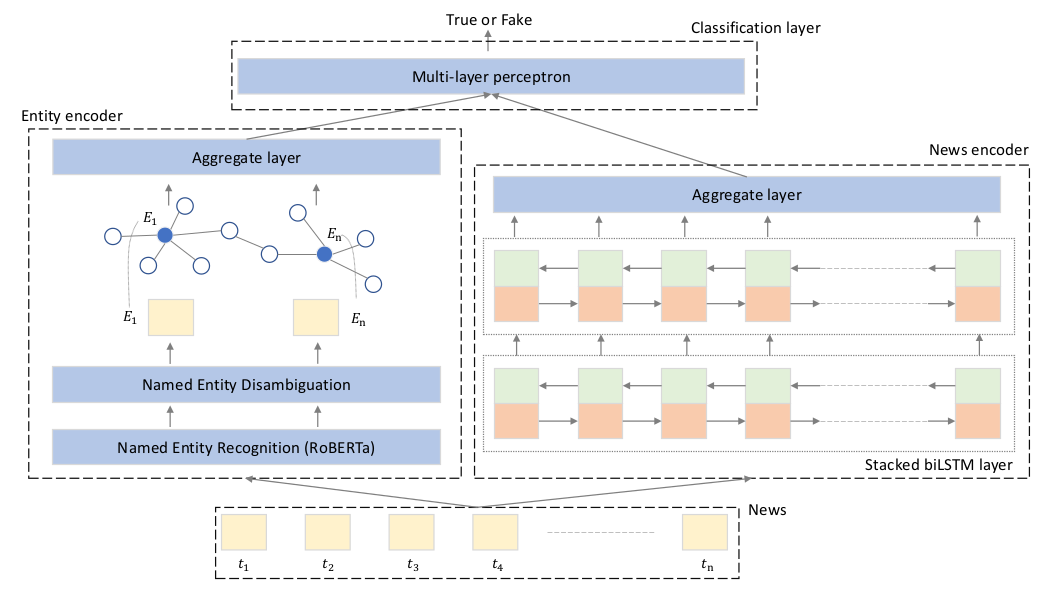
\includegraphics[scale=0.45]{img/deap_fake_framework.png}
	\caption{From DEAP-FAKED paper - Illustration of the proposed DEAP-FAKED framework. The left sub-figure shows the entity encoder module. The right sub-figure shows the news encoder module. The top sub-figure is the Fake News classifier module. The bottom shows the tokenized news as the input to the entity encoder and news encoder.}
\end{figure}

The dataset used for \textit{DEAP-FAKED} framework can be described as following:

\begin{itemize}
\item \textbf{Fake News dataset:} The first dataset is the Kaggle Fake News dataset, which consists of 20,387 news items, having a near equal combination of true and Fake News. The news covers several domains such as Politics, Business, and Technology.
The complete pre-processing step brought down the news item count to  $\sim$14k with a distribution of 60\% - 40\% of true and Fake News classes, respectively.They called this dataset KFN-UB.\\
The second dataset is CoAID, which contains diverse COVID-19 healthcare misinformation, including Fake News from websites and social platforms. CoAID includes 4,251 news items. After pre-processing it only 632 news item and called CoAID-UB.
\item \textbf{Knowledge Graph:} the framework uses Wikidata5M as a knowledge graph, it is created by only considering the "valid" facts, where the validity is confirmed if all entities and relations in the fact have a Wikipedia article and long description.
\end{itemize}

As for the evaluation procedure, they chose five baseline models for comparison with \textit{DEAP-FAKED} framework: ExtraTreeClassifier, LSTM, SentRoBERTa, StackedBiLSTM, and StackedBiLSTM.

\begin{figure}[H]
	\centering
	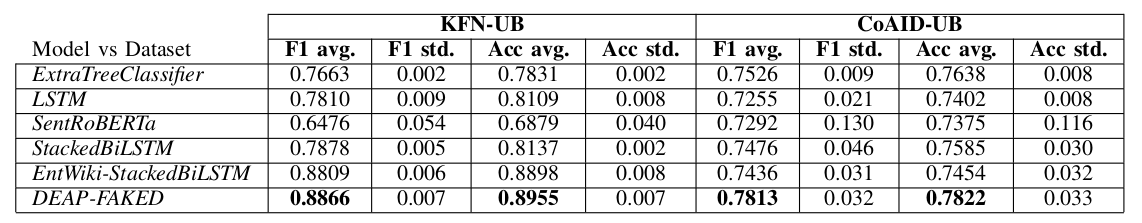
\includegraphics[scale=0.4]{img/deap_faked_evaluation.png}
	\caption{From DEAP-FAKED paper - Performance score of the models detailed in the paper is presented here. For each of the dataset, we report F1 macro and Accuracy metric values. We present average and standard deviation of the performance observed after performing 3 trials with different starting seed. For both the datasets, DEAP-FAKED reports the best performance value.}
\end{figure}

As evident by the results, \textit{DEAP-FAKED} reports the highest score on both of the datasets.


\subsection{Hierarchical Propagation based fake news detection \cite{shu2020hierarchical}}
In a paper wrote by \textit{Kai Shu}, \textit{Deepak Mahudeswaran}, \textit{Suhang Wang}, and \textit{Huan Liu} with the name of \textit{Hierarchical Propagation Networks for Fake News Detection: Investigation and Exploitation}, the detection of fake news can be done by looking at the correlation between news and the hierarchical characteristics of a social network.\\

The datasets used for this study were the public fake news repository \textit{FakeNewsNet} \cite{shu2018fakenewsnet} that contains data related to different fact-checking websites that offers news content, social context and dynamic information. In addition, they used the data from fact-checking websites \textit{GossipCop} and \textit{PolitiFact} that contains news articles with labels annotated by professional journalists. News content includes meta attributes of the news like body text, he social context includes the related user interactions with the news like posting, sharing, commenting on Twitter, and dynamic information contains the timestamps of user's interactions.\\

After collecting all of this data, building a hierarchical propagation network was the next step. First of all they defined two major levels of the hierarchy: 

\begin{itemize}
\item \textbf{Micro-level:} involves users conversations towards news pieces on social media over time. It contains rich information of user opinions towards news pieces.
\item \textbf{Macro-level:} encompasses information on tweets posting pattern and information sharing pattern. It represents the global propagation of information through a cascade of re-tweets.
\end{itemize}

\begin{figure}[H]%
	\centering
	\begin{subfigure}{.5\textwidth}
		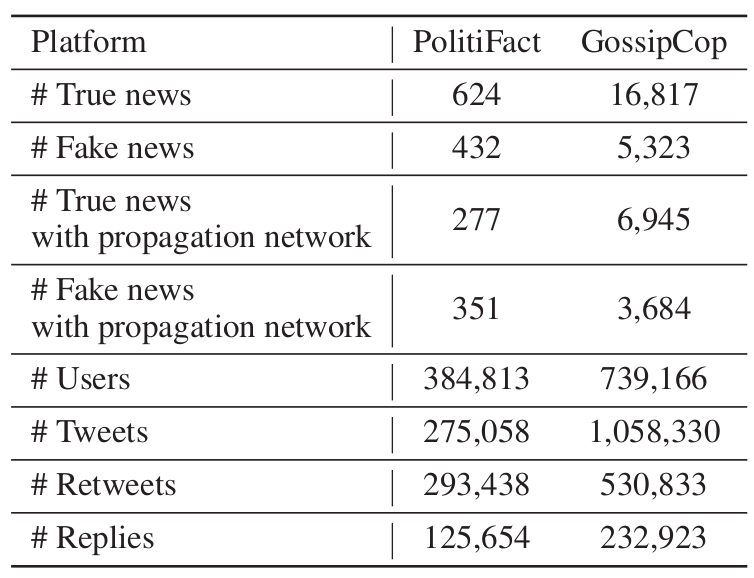
\includegraphics[width=.9\linewidth, height=7cm]{img/fake_news_net_content.png}
		\caption{The statistics of FakeNewsNet}
	\end{subfigure}%
	\begin{subfigure}{.5\textwidth}
		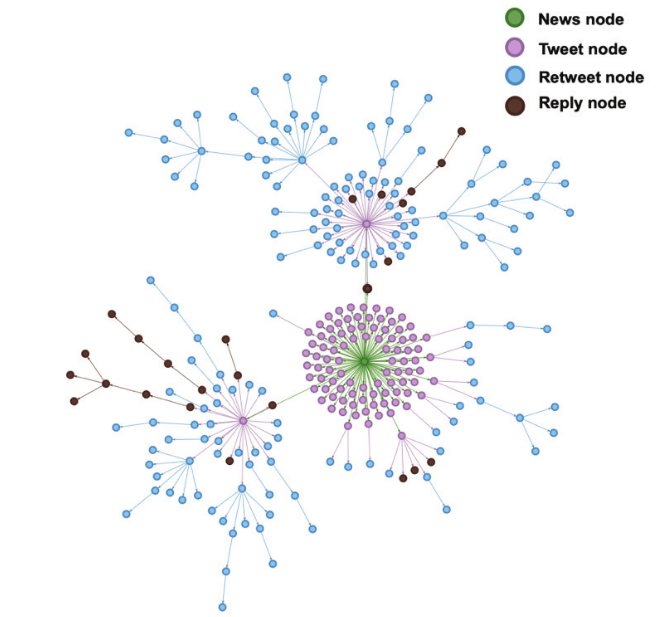
\includegraphics[width=.9\linewidth, height=7cm]{img/hierarchy_network.png}
		\caption{An example of the hierarchical propagation network of a fake news piece fact-checked by Politifact. It consists of two types: macro-level and micro-level. The macro-level propagation network includes the news nodes, tweet nodes, and retweet nodes. The micro-level propagation network indicates the conversation tree represented by cascade of reply nodes.}
	\end{subfigure}
	\caption{From the \textit{Hierarchical Propagation Networks for Fake News Detection: Investigation and Exploitation} paper}%
\end{figure}



In both these levels they used \textit{Structural Analysis} to identify patterns in conversations, \textit{Temporal Analysis} to understand the exchange of opinions in terms of time. For the Micro-level they added a \textit{Linguistic Analysis} to inference the sentiment of people around news pieces, thus obtaining linguistic features for statistical comparison.\\

To evaluate the performance of fake news detection of the model they choose randomly 80\% of news articles for training and the remaining 20\% for testing. The results shows high scores for both datasets:

\begin{figure}[H]
	\centering
	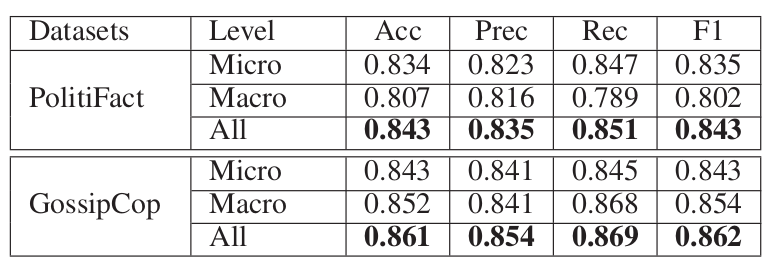
\includegraphics[scale=0.4]{img/hierarchical_evaluation_results.png}
	\caption{From the \textit{Hierarchical Propagation Networks for Fake News Detection: Investigation and Exploitation} paper - Evaluation of the model}
\end{figure}


\subsection{Perplexity based fake news detection \cite{lee2021towards}}
In March 2021, \textit{Nayeon Lee}, \textit{Yejin Bang}, \textit{Andrea Madotto}, \textit{Madian Khabsa}, and \textit{Pascale Fung} published a paper called \textit{Towards Few-Shot Fact-Checking via Perplexity} where they propose a new approach of the powerful transfer learning ability of a language model via a perplexity score. Using a method called \textit{few-shot learning}, they built a model that outperforms major class baseline models by more than 10\% on the F1-Macro metric score.\\

\begin{figure}[H]
	\centering
	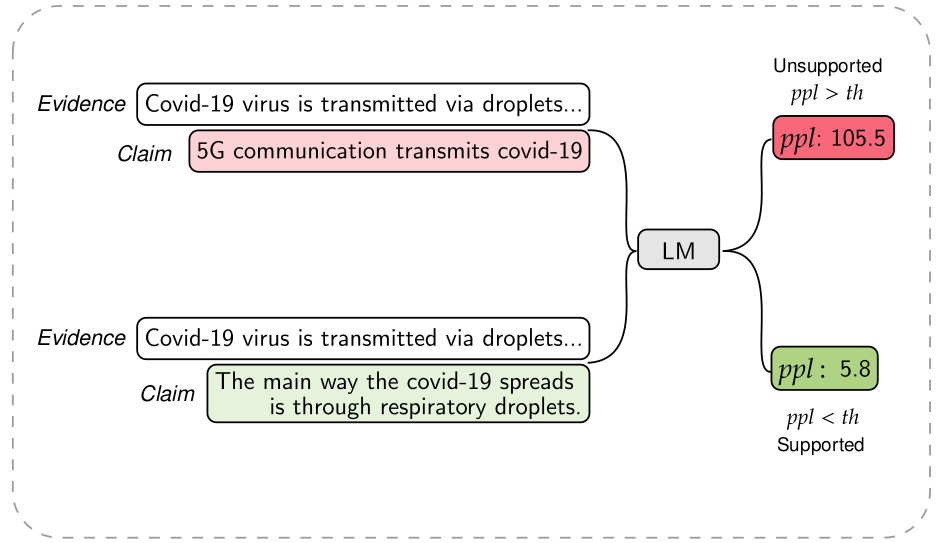
\includegraphics[scale=0.3]{img/perplexity_example.png}
	\caption{From the \textit{Towards Few-Shot Fact-Checking via Perplexity} paper - Illustration of our simple yet effective perplexity-based approach. Few-shot data samples are used to find the optimal perplexity threshold th that separates Unsupported claims from Supported claims.}
\end{figure}

\textit{Few-Shot Learning} refers to the technique of feeding a machine learning model with a very small amount of training data to guide its predictions, like a few examples at inference time, as opposed to standard fine-tuning techniques which require a relatively large amount of training data for the pre-trained model to adapt to the desired task with accuracy.\\
In NLP, \textit{Few-Shot Learning} can be used with Large Language Models (LMs), which have learned to perform a wide number of tasks implicitly during their pre-training on large text datasets. This enables the model to generalize, that is to understand related but previously unseen tasks, with just a few examples.\\

Perplexity is a commonly used metric for measuring the performance of LMs. It is defined as the inverse of the probability of the test set normalized by the number of words:

\begin{figure}[H]
	\centering
	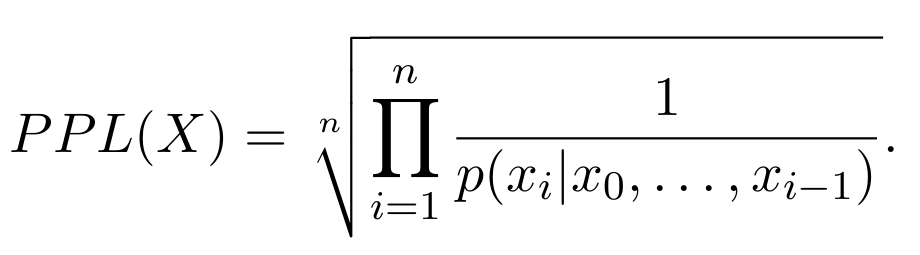
\includegraphics[scale=0.2]{img/perplexity_equation.png}
	\caption{Perplexity score}
\end{figure}

Another way of interpreting perplexity is as a measure of the likelihood of a given test sentence with reference to the training corpus.\\

In this paper the goal is to determine the veracity of a claim given some evidence, for this they define a {claim, evidence} pair. The label \emph{Supported} is assigned when relevant evidence exists that supports the claim, and \emph{Unsupported} label for the opposite case.\\
\emph{Unsupported} claims on average have higher perplexity than \emph{Supported} claims. For example, \emph{Supported} claim "Washing hands prevents the spread of diseases" has a perplexity value of 96.74, whereas the \emph{Unsupported} claim "All dogs speak English fluently" has a much higher perplexity value of 328.23. 

\begin{figure}[H]
	\centering
	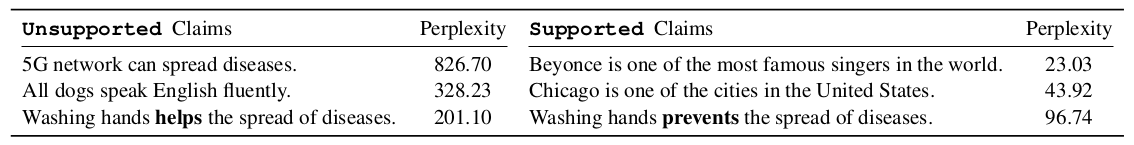
\includegraphics[scale=0.43]{img/supported_unsupported_perplexity.png}
	\caption{From the \textit{Towards Few-Shot Fact-Checking via Perplexity} paper - Relations between veracity of claim and perplexity. Unsupported claims have higher perplexity compared to Supported claims. Note that the perplexity score listed here is using GPT2-base on each of the claims.}
\end{figure}

The datasets used in this experiment are:

\begin{itemize}
\item \textbf{Covid19-Scientific:} a new test set constructed by collecting COVID-19-related myths and scientific truths labeled by reliable sources like MedicalNewsToday, the Centers for Disease Control and Prevention (CDC), and the World Health Organization (WHO). The set contains 172 claims with labels \emph{(Supported, Unsupported)} obtained from the aforementioned reliable sources.
\item \textbf{Covid19-Social:} a collection of 340 COVID-19-related claims fact-checked by journalists from Politifact.com. Unlike the Covid19-Scientific dataset, it contains non-scientific and socially-related claims, such as "For the coronavirus, the death rate in Texas, per capita of 29 million people, we're one of the lowest in the country".
\item \textbf{FEVER:} Fact Extraction and Verification (FEVER) is a publicly released large-scale dataset generated by altering sentences extracted from Wikipedia to promote research on fact-checking systems.
\end{itemize}

For the models created for this perplexity based experiment they used one unidirectional LM and one masked LM:

\begin{itemize}
\item $PPL_{GPT2-B}$ : a single-parameter classifier based on perplexity from GPT2-base \cite{radford2019language} (unidirectional LM)
\item $PPL_{BERT-B}$ : a single-parameter classifier based on perplexity from BERT-base \cite{devlin2018bert} (Masked LM)
\end{itemize}

As for baseline models they finetuned pre-trained Transformer-based \cite{vaswani2017attention} in order to build a classifier, which is a common approach used to achieve many state-of-the-art results in the literature.\\

Moving to the experimental setup, they used the \textit{Few-Shot} technique in order to validate or train the models. Given $N_D$ as the size of the dataset $D$, we do an $n$-shot experiment with $n$ samples from $D$ as a "validation set" for our perplexity-based approach or as a "training set" for the fine-tuning approach, and the remainder ($N_D - n$) as a test set. For example in the 2-shot experiment using the Covid19-Social dataset (340 samples), we have two training samples and 338 test samples.\\
They took into consideration the accuracy and the F1-Macro metrics for the evaluation. Because the datasets are unbalanced, they mainly consider the F1-Macro score over accuracy as an overall evaluation.\\


\begin{figure}[H]
	\centering
	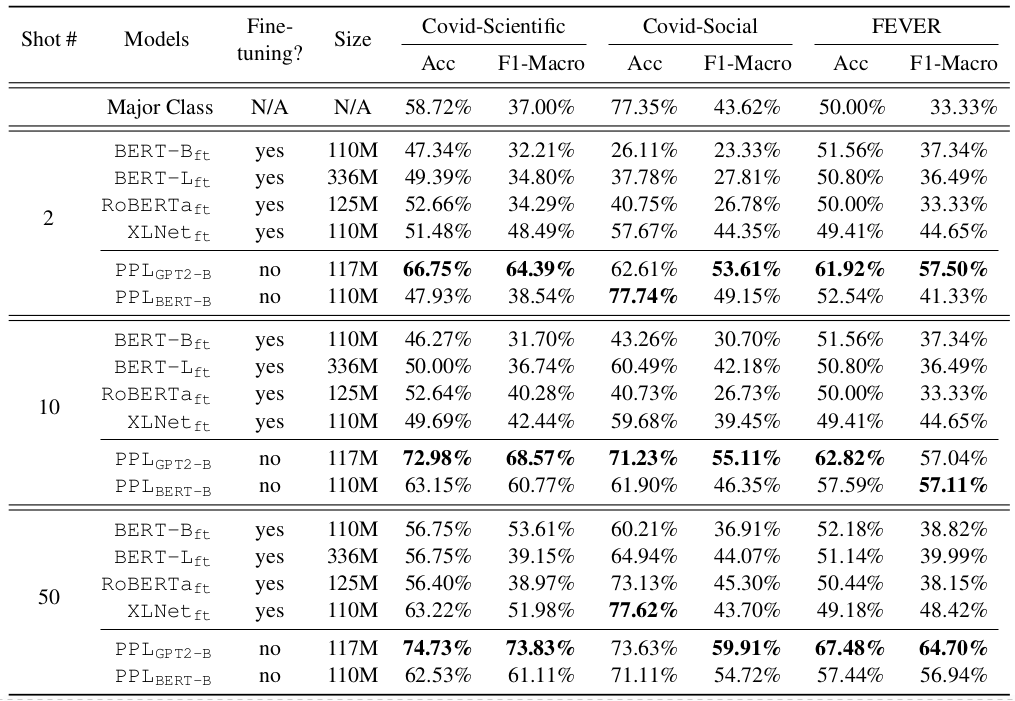
\includegraphics[scale=0.43]{img/few_shots_perplexity_evaluation.png}
	\caption{From the \textit{Towards Few-Shot Fact-Checking via Perplexity} paper - Results comparison among perplexity-based classifiers and fine-tuned classifiers in 2-shot, 5-shot and 10-shot settings across three different tasks. Models whose names start with PPL are our proposed perplexity-based classifiers. Major Class is a reference to evaluate classifier performance. All test results reported are mean values of three trials with randomly selected n-shot training samples from the dataset, where $n={2, 10, 50}$.}
\end{figure}

We can observe that the perplexity-based classifiers, especially $PPL_{GPT2-B}$, outperform all Major Class baselines across all
tasks in all settings. For instance, $PPL_{GPT2-B}$ outperforms the Major Class by a great margin of
16\% and 36.8\% on accuracy and F1-Macro scores. Evidence conditioned perplexity scores are capable of providing signals regarding the veracity of the the given claim.

\subsection{Other approaches}




\chapter{Conclusion}


\chapter{Perspectives}


\bibliographystyle{abbrv}
\bibliography{ref}


\end{document}
